\chapter{Binary Decision Diagrams}
\begin{figure}[h!]
\centering
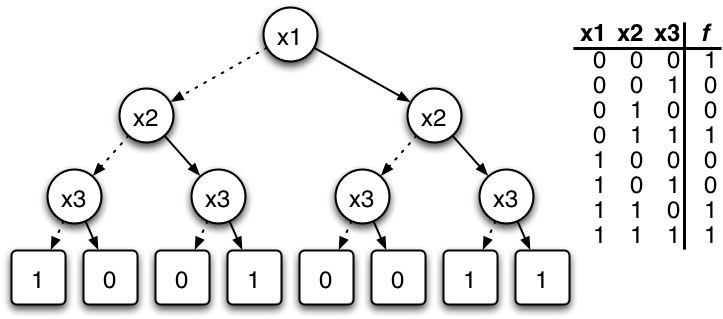
\includegraphics[width=4in]{binarydd/bdd-tree.png}
\caption{Binary decision tree and truth table 
for the function $
f(x_1, x_2,x_3)=
\bar{x}_1(x_2+\bar{x}_3)  + x_1 x_2 $ }
\label{fig-bdd-tree}
\end{figure}

\begin{figure}[h!]
\centering
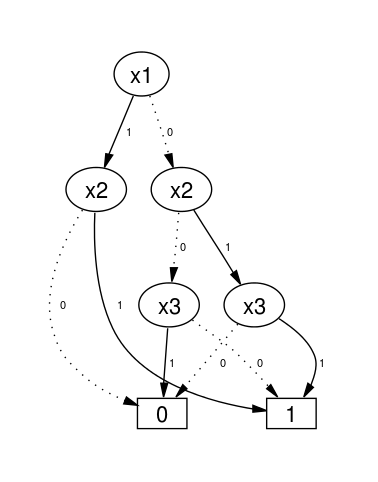
\includegraphics[width=2in]{binarydd/bdd.png}
\caption{BDD for the function $f$
of Fig.\ref{fig-bdd-tree}.} 
\label{fig-bdd}
\end{figure}

This chapter is based
on Wikipedia article Ref.\cite{wiki-bdd}.

Binary Decision Diagrams (BDDs)
can be understood as a special
case of Decision Trees (dtrees).
We will
assume
that the reader has read
Chapter \ref{ch-dtree} 
on dtrees before
reading this chapter.

Both Figs.\ref{fig-bdd-tree}
and \ref{fig-bdd} were taken
from the aforementioned Wikipedia article. They
give a simple example of a function
$f:\bool^3\rarrow\bool$
represented in
Fig.\ref{fig-bdd-tree} as a
{\bf binary decision tree}
 and in Fig.\ref{fig-bdd} as a {\bf binary
decision diagram (BDD)}.
The goal 
of this chapter is
to find for each  of those 
figures a bnet with
the same graph structure.

We begin by noting
that the function
$f:\bool^3\rarrow\bool$
is a special case
of a probability
distribution
$P:\bool^3\rarrow[0,1]$.
In fact,
if we restrict $P$ to 
be deterministic, then
$P_{det}:\bool^3\rarrow\bool$
has the same domain
and range as $f$.
Henceforth,
we will refer to
$f(x_1,x_2,x_3)$
as $P(x_1,x_2,x_3)$,
keeping in mind that
we are restricting our
attention to deterministic
probability distributions. 

If we apply the chain
rule for conditional
probabilities to $P(x_1,x_2,x_3)$,
we get
\beq
P(x_1, x_2, x_3)=
P(x_3|x_1, x_2)P(x_2|x_1)P(x_1)
\;,
\eeq
which can be represented by the bnet:

\beq
\xymatrix{
\rvx_1\ar[d]\ar@/^1pc/[dd]\\
\rvx_2\ar[d]\\
\rvx_3
}
\label{eq-bdd-full-bnet}
\eeq
But
in Chapter \ref{ch-dtree},
we learned how
to represent
the bnet
of Eq.(\ref{eq-bdd-full-bnet})
as the bnet tree 
Eq.(\ref{eq-bdd-full-tree}).
In that tree,
the nodes
pose questions
with 3 possible answers $0,1,null$.
In Eq.(\ref{eq-bdd-full-tree}),
$x_2|a?$ stands for 
``what is $x_2$ if $x_1=a?$" and
$x_3|a,b?$ stands for ``what is 
$x_3$ if $x_1=a,x_2=b$?".



\beq
\xymatrix{
\ul{x_1?}\ar[d]\ar[dr]
\\
\ul{x_2|0?}\ar[d]\ar[dr]
&\ul{x_2|1?}\ar[dr]\ar[drr]
\\
\ul{x_3|00?}
&\ul{x_3|01?}
&\ul{x_3|10?}
&\ul{x_3|11?}
}
\label{eq-bdd-full-tree}
\eeq

The node TPMs, printed in blue,
for the bnet of Eq.(\ref{eq-bdd-full-tree})
are as follows.
If $x_1,x_2, x_3\in \{0,1,null\}$
and $a,b\in \bool$, then

\beq\color{blue}
P(\ul{x_1?}=x_1)=
\left\{
\begin{array}{ll}
P_{\rvx_1}(x_1)&\text{if $x_1\in \bool$}
\\
0&\text{if $x_1=null$}
\end{array}
\right.
\eeq


\beq\color{blue}
P(\ul{x_2|a?}=x_2\cond \ul{x_1?}=x_1)=
\left\{
\begin{array}{ll}
P_{\rvx_2|\rvx_1}(x_2|a)&\text{if $x_1=a$}
\\
\indi(x_2=null)&\text{otherwise}
\end{array}
\right.
\eeq

\beq\color{blue}
P(\ul{x_3|a,b?}=x_3\cond \ul{x_2|b?}=x_2)=
\left\{
\begin{array}{ll}
P_{\rvx_3|\rvx_1,\rvx_2}
(x_3|a,b)&\text{if $(x_1,x_2)=(a,b)$}
\\
\indi(x_3=null)&\text{otherwise}
\end{array}
\right.
\eeq
The bnet shown in
Eq.(\ref{eq-bdd-full-tree})
contains
the same info
and has 
the same graph structure
as the binary decision
tree Fig.\ref{fig-bdd-tree}.
As when we were
converting dtrees to
their image bnets, the
info in the endpoint nodes
of Fig.\ref{fig-bdd-tree}
is implicit
in the node
TPMs
of the image bnet
Eq.(\ref{eq-bdd-full-tree}).
If one
wants to make the endpoint  node info
more explicit in the image bnet,
one can add it to the descriptors of
the state names of the leaf nodes
of the image bnet.
For example,
one can add descriptors 
``gives $f=0$"
or ``gives $f=1$" to the
 ``0" or ``1" states of
those leaf nodes.

The BDD shown in
Fig.\ref{fig-bdd}
emphasizes the
fact that

\beq
P(x_1,x_2,x_3|x_1=1)=P(x_2|x_1=1)=x_2
\;.
\eeq
The BDD of Fig.\ref{fig-bdd}
corresponds to
the bnet of
Eq.(\ref{eq-bdd-bnet}).

\beq
\xymatrix{
\ul{x_1?}\ar[d]\ar[dr]
\\
\ul{x_2|0?}\ar[d]\ar[dr]
&\ul{x_2|1?}
\\
\ul{x_3|00?}
&\ul{x_3|01?}
&\bullet
&\bullet
}
\label{eq-bdd-bnet}
\eeq

\hrule
What happens
if we consider an $f$ for which
$P(x_3|x_1, x_2)=P(x_3|x_2)$ so that
one of the arcs of the
fully connected bnet Eq.(\ref{eq-bdd-full-bnet})
is unnecessary?
In that case,

\beq
P(x_1, x_2, x_3)=
P(x_3| x_2)P(x_2|x_1)P(x_1)
\;,
\eeq
which can be represented by the 
Markov chain bnet:

\beq
\xymatrix{
\rvx_1\ar[d]\\
\rvx_2\ar[d]\\
\rvx_3
}
\;.
\label{eq-bdd-markov}
\eeq

Following the prescriptions
of Chapter \ref{ch-dtree}, we
can represent
the bnet
of Eq.(\ref{eq-bdd-markov})
as the bnet tree 
Eq.(\ref{eq-bdd-markov-tree}).
In that tree,
the nodes
pose questions
with 3 possible answers $0,1,null$.

\beq
\xymatrix{
\ul{x_1?}\ar[d]\ar[dr]
\\
\ul{x_2|0?}\ar[d]\ar[dr]
&\ul{x_2|1?}\ar[dr]\ar[drr]
\\
\ul{x_3|\_,0?}
&\ul{x_3|\_,1?}
&\ul{x_3|\_,0?}
&\ul{x_3|\_,1?}
}
\label{eq-bdd-markov-tree}
\eeq



